% ─────────────────────────────────────────────────────────────────────────────
% How it's all connected — the game-engine hosting & analytics front door
% TeX backend (Tectonic). Build: node tools/pdf/tex-build.mjs docs/pdf/hosting.tex
% Authored from docs/HOSTING.md.
% ─────────────────────────────────────────────────────────────────────────────
\documentclass[11pt]{article}

\usepackage[a4paper,margin=1in]{geometry}
\usepackage{graphicx}
\usepackage{xcolor}
\usepackage{booktabs}
\usepackage{enumitem}
\usepackage{titlesec}
\usepackage{fancyhdr}
\usepackage{listings}
\usepackage{microtype}
\usepackage{tikz}
\usetikzlibrary{arrows.meta,positioning,shapes.geometric}
\usepackage[colorlinks=true,linkcolor=accent,urlcolor=accent,citecolor=accent]{hyperref}

\newcommand{\doctitle}{How It's All Connected --- the Hosting \& Analytics Front Door}

% ── palette ──
\definecolor{ink}{HTML}{1B1F24}
\definecolor{accent}{HTML}{0B7285}
\definecolor{soft}{HTML}{F1F3F5}
\definecolor{line}{HTML}{CED4DA}
\definecolor{good}{HTML}{2B8A3E}
\definecolor{warn}{HTML}{E8590C}

% ── headings ──
\titleformat{\section}{\Large\bfseries\color{accent}}{\thesection}{0.6em}{}
\titleformat{\subsection}{\large\bfseries\color{ink}}{\thesubsection}{0.6em}{}
\titlespacing*{\section}{0pt}{1.4em}{0.5em}

% ── footer ──
\pagestyle{fancy}\fancyhf{}
\renewcommand{\headrulewidth}{0pt}
\renewcommand{\footrulewidth}{0.4pt}
\fancyfoot[L]{\small\color{ink}game-engine · hosting}
\fancyfoot[R]{\small\thepage}

% ── code ──
\lstset{
  basicstyle=\ttfamily\small,
  backgroundcolor=\color{soft},
  frame=single, rulecolor=\color{line},
  breaklines=true, columns=fullflexible, showstringspaces=false,
  keywordstyle=\color{accent}\bfseries, commentstyle=\color{gray},
  xleftmargin=0.6em, framexleftmargin=0.6em,
}

% ── callout ──
\newcommand{\callout}[1]{%
  \par\medskip\noindent
  \colorbox{soft}{\parbox{\dimexpr\linewidth-2\fboxsep\relax}{\color{ink}#1}}%
  \par\medskip}

% ── tikz layer style ──
\tikzset{
  layer/.style={
    draw=line, fill=soft, rounded corners=4pt, line width=0.7pt,
    text width=0.80\linewidth, align=left, inner sep=7pt, font=\small\color{ink}},
  head/.style={draw=accent, fill=accent!10, line width=1pt},
  flow/.style={-{Stealth[length=3mm]}, line width=0.9pt, color=accent},
  side/.style={font=\scriptsize\itshape\color{gray}},
}

% give justified paragraphs room to avoid overfull boxes around long code / URL spans
\setlength{\emergencystretch}{3em}\tolerance=1200

\title{\color{accent}\doctitle}
\author{Engine · TeX backend}
\date{\today}

\begin{document}
\maketitle
\thispagestyle{fancy}

\section{The one-paragraph picture}
This is how a person typing \texttt{play.funstackstudios.com} on their phone ends up
playing a game --- and how their tap flows back to you as analytics. It is the
\emph{outside} of the engine: the registrar, Railway, the hub, and the per-game
deployments. A custom domain only works when \textbf{four independent layers} all
agree --- DNS, the certificate, the edge route, and the app itself. Any one can be
green while another is broken, so ``it doesn't work'' is never enough: you check
each hop. (For the \emph{inside} --- how a game is built --- see \texttt{docs/ENGINE.md}.)

\callout{\textbf{The trap this rig is built to catch:} DNS is propagated, the cert
is \textsc{valid}, Railway's API says the domain is fine --- yet the edge still
answers with a fallback \texttt{404} (\texttt{x-railway-fallback: true}) because it
never bound the hostname to the service. The fix is a \emph{redeploy of the bound
service}, not a DNS change. The \texttt{domain-doctor} skill automates the whole
diagnosis.}

\section{The four layers}

\begin{center}
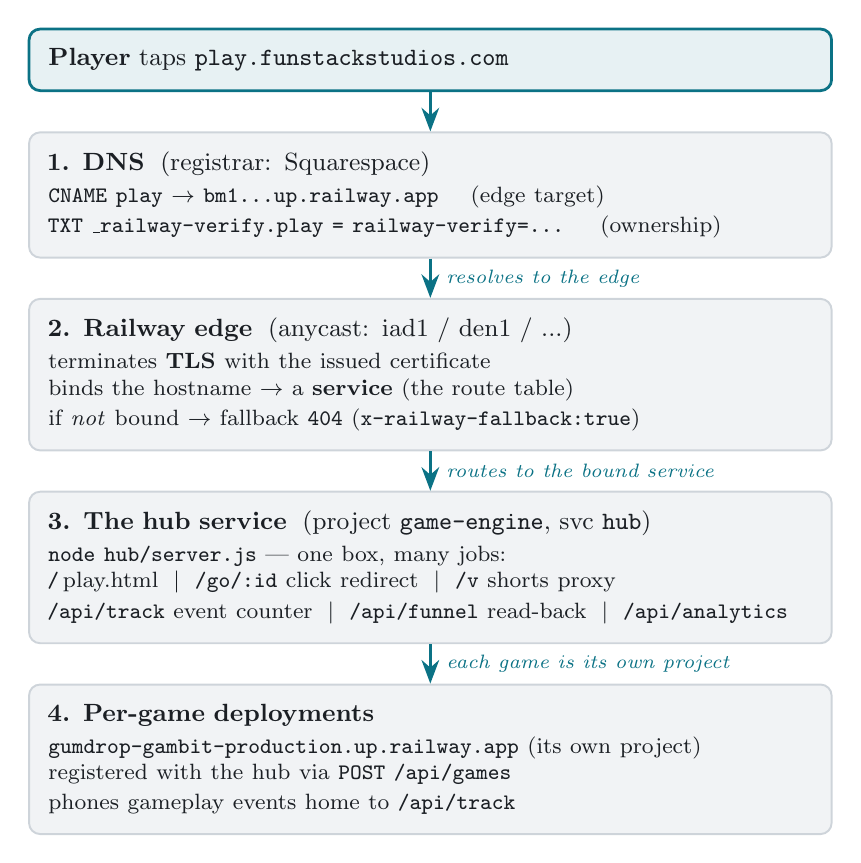
\begin{tikzpicture}[node distance=0.5cm]
  \node[layer, head] (player) {\textbf{Player} taps \texttt{play.funstackstudios.com}};
  \node[layer, below=of player] (dns)
    {\textbf{1. DNS} \;(registrar: Squarespace)\\[2pt]
     \footnotesize \texttt{CNAME play $\to$ bm1...up.railway.app} \quad(edge target)\\
     \footnotesize \texttt{TXT \_railway-verify.play = railway-verify=...} \quad(ownership)};
  \node[layer, below=of dns] (edge)
    {\textbf{2. Railway edge} \;(anycast: iad1 / den1 / ...)\\[2pt]
     \footnotesize terminates \textbf{TLS} with the issued certificate\\
     \footnotesize binds the hostname $\to$ a \textbf{service} (the route table)\\
     \footnotesize if \emph{not} bound $\to$ fallback \texttt{404} (\texttt{x-railway-fallback:true})};
  \node[layer, below=of edge] (hub)
    {\textbf{3. The hub service} \;(project \texttt{game-engine}, svc \texttt{hub})\\[2pt]
     \footnotesize \texttt{node hub/server.js} --- one box, many jobs:\\
     \footnotesize \texttt{/}\,play.html \;\textbar\; \texttt{/go/:id} click redirect \;\textbar\; \texttt{/v} shorts proxy\\
     \footnotesize \texttt{/api/track} event counter \;\textbar\; \texttt{/api/funnel} read-back \;\textbar\; \texttt{/api/analytics}};
  \node[layer, below=of hub] (games)
    {\textbf{4. Per-game deployments}\\[2pt]
     \footnotesize \texttt{gumdrop-gambit-production.up.railway.app} (its own project)\\
     \footnotesize registered with the hub via \texttt{POST /api/games}\\
     \footnotesize phones gameplay events home to \texttt{/api/track}};

  \draw[flow] (player) -- (dns);
  \draw[flow] (dns) -- (edge) node[side, midway, right=2pt] {resolves to the edge};
  \draw[flow] (edge) -- (hub) node[side, midway, right=2pt] {routes to the bound service};
  \draw[flow] (hub) -- (games) node[side, midway, right=2pt] {each game is its own project};
\end{tikzpicture}
\end{center}

\subsection{1 · DNS --- the registrar (Squarespace)}
The apex \texttt{funstackstudios.com} is registered at Squarespace, so the public
hostname is configured there as custom DNS records. A Railway custom domain needs
exactly two:

\begin{center}
\begin{tabular}{@{}llp{6.2cm}@{}}
\toprule
Type & Name & Purpose \\
\midrule
\texttt{CNAME} & \texttt{play} & points the hostname at Railway's edge target \\
\texttt{TXT} & \texttt{\_railway-verify.play} & proves ownership so Railway issues the cert \\
\bottomrule
\end{tabular}
\end{center}

\noindent DNS belongs to the \textbf{owner} --- these are the only steps a human does
by hand. The \texttt{TXT} unblocks certificate issuance; once the cert is
\textsc{valid}, Railway stops requiring it. \textbf{Don't re-add the domain on Railway
to ``fix'' things} --- each re-add can mint a \emph{new} CNAME target and force you to
redo the DNS.

\subsection{2 · Railway edge --- TLS + the route binding}
The anycast edge does two separate jobs, and \emph{either} can be green while the
other is broken:
\begin{itemize}[noitemsep,leftmargin=1.2em]
  \item \textbf{Certificate} --- issued once the \texttt{\_railway-verify} TXT checks
        out. Until then you get a TLS warning, not a 404.
  \item \textbf{Route binding} --- maps the hostname to the \texttt{hub} service. This
        is the layer DNS dashboards can't show. When it's stuck, the edge answers from
        a \emph{fallback} app and sets \texttt{x-railway-fallback: true}. The status
        code lies; that header is the only tell. \textbf{The fix is a redeploy of the
        bound service}, which makes the edge re-read its route table --- no DNS change.
\end{itemize}

\subsection{3 · The hub service --- one box, many jobs}
A single Railway project (\texttt{game-engine}) running one service (\texttt{hub},
\texttt{node hub/server.js}). It is both the public storefront and the analytics sink:

\begin{center}
\begin{tabular}{@{}lp{8.6cm}@{}}
\toprule
Route & Job \\
\midrule
\texttt{/} & \texttt{play.html} --- the mobile game list; each card's thumb is the static file \texttt{hub/public/thumbs/<id>.jpg} (360$\times$360) \\
\texttt{/go/:id} & logs a \textbf{click} (with \texttt{utm\_source}) then 302-redirects to the game \\
\texttt{/v?src=} & proxies each game's shorts \emph{same-origin} (byte-range mp4) so the feed plays reliably \\
\texttt{/api/track} & open-CORS, server-side, ad-blocker-proof event counter \\
\texttt{/api/funnel} & reads back clicks + events \\
\texttt{/api/analytics} & per-game code / asset / cost (from GitHub) \\
\bottomrule
\end{tabular}
\end{center}

\noindent State lives in \texttt{store.js}, a tiny KV on a Railway \textbf{volume} (the
games list, funnel counts), so a restart paints instantly.

\subsection{4 · Per-game deployments}
Each game is its \emph{own} Railway project (e.g.\ \texttt{gumdrop-gambit} $\to$
\texttt{gumdrop-gambit-\allowbreak production\allowbreak.up.railway.app}), auto-deploying from its GitHub repo.
A game joins the hub by calling \texttt{POST /api/games} with its \texttt{id},
\texttt{url}, and hosted \texttt{shorts} --- \emph{without} a hub code change. From then
on the hub lists it, proxies its shorts, and collects its events.

\section{The loop it creates --- shorts $\to$ analytics}
This hosting rig is what makes the flywheel measurable end to end.

\begin{center}
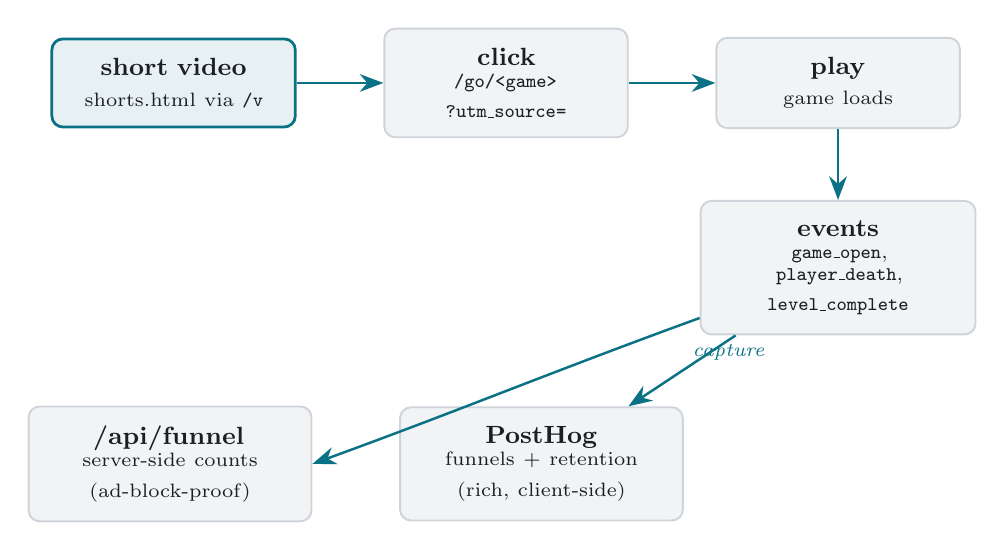
\begin{tikzpicture}[node distance=0.9cm and 1.1cm, every node/.style={font=\footnotesize}]
  \node[layer, head, text width=2.6cm, align=center] (short) {\textbf{short video}\\ \scriptsize shorts.html via \texttt{/v}};
  \node[layer, text width=2.6cm, align=center, right=of short] (click) {\textbf{click}\\ \scriptsize \texttt{/go/<game>}\\ \scriptsize \texttt{?utm\_source=}};
  \node[layer, text width=2.6cm, align=center, right=of click] (play) {\textbf{play}\\ \scriptsize game loads};
  \node[layer, text width=3.0cm, align=center, below=of play] (events) {\textbf{events}\\ \scriptsize \texttt{game\_open},\\ \scriptsize \texttt{player\_death},\\ \scriptsize \texttt{level\_complete}};
  \node[layer, text width=3.1cm, align=center, below left=0.9cm and 0.2cm of events] (posthog) {\textbf{PostHog}\\ \scriptsize funnels + retention\\ \scriptsize (rich, client-side)};
  \node[layer, text width=3.1cm, align=center, left=of posthog] (funnel) {\textbf{/api/funnel}\\ \scriptsize server-side counts\\ \scriptsize (ad-block-proof)};

  \draw[flow] (short) -- (click);
  \draw[flow] (click) -- (play);
  \draw[flow] (play) -- (events);
  \draw[flow] (events) -- (posthog) node[side,midway,above right] {capture};
  \draw[flow] (events) to[out=200,in=20] (funnel.east);
\end{tikzpicture}
\end{center}

\begin{itemize}[noitemsep,leftmargin=1.2em]
  \item \textbf{PostHog} (public \texttt{phc\_...} key) captures the rich client funnel
        (\texttt{\$pageview $\to$ game\_open $\to$ level\_start $\to$ level\_complete},
        broken down by \texttt{utm\_source}) and retention.
  \item \textbf{\texttt{/api/track} $\to$ \texttt{/api/funnel}} is the first-party
        server-side truth that survives ad-blockers (which eat $\sim$10--40\% of mobile
        client events). Reconcile the two to size the blind spot.
  \item The same gameplay events double as \textbf{eval signal} --- death heatmaps,
        difficulty / reach calibration. See the \texttt{analytics} skill.
\end{itemize}

\section{Health-checking the front door --- \texttt{domain-doctor}}
Run any time the public domain misbehaves or after a DNS change. It walks all four
layers, prints a pass/fail table, and with \texttt{--fix} clears a stuck edge binding
by redeploying the bound service.

\begin{lstlisting}[language=bash]
node scripts/domain-doctor.mjs play.funstackstudios.com \
  --project game-engine --health /health
\end{lstlisting}

\begin{center}
\begin{tabular}{@{}clp{7.2cm}@{}}
\toprule
\# & Hop & Green means \\
\midrule
1 & \textbf{DNS CNAME} & hostname resolves to a Railway edge target (via DoH; \texttt{dig} isn't installed) \\
2 & \textbf{DNS TXT verify} & the \texttt{\_railway-verify} record is present (only needed until the cert is valid) \\
3 & \textbf{Railway cert} & \texttt{certificateStatus == VALID} \\
4 & \textbf{Railway DNS} & every \texttt{dnsRecords} entry is \texttt{PROPAGATED} \\
5 & \textbf{Edge serving} & HTTPS \texttt{200} \emph{and} no \texttt{x-railway-fallback} header \\
6 & \textbf{App health} & the app answers on \texttt{--health <path>} \\
\bottomrule
\end{tabular}
\end{center}

\callout{\textbf{Don't skip the ladder.} A correct CNAME with \emph{no cert} = TLS
error, not a 404. A valid cert with an \emph{unbound edge} = a clean \texttt{200} from
the \emph{fallback} app, not yours. A bound edge with a \emph{dead app} = \texttt{502}.
Checking the app's native \texttt{*.up.railway.app} URL isolates ``app is down'' from
``domain isn't wired.''}

\vfill
\noindent{\footnotesize Source: \texttt{docs/HOSTING.md} · skill: \texttt{domain-doctor}
(\texttt{scripts/domain-doctor.mjs}) · this PDF is typeset by the engine's TeX backend
(Tectonic).}

\end{document}
